\documentclass{article}
\usepackage[utf8]{inputenc}
\usepackage{graphicx} % Required for inserting img
\usepackage{amsmath}
\usepackage{multirow}
\usepackage{fullpage}
\usepackage{amsfonts}

\usepackage{xcolor}

\title{David's experiments}
\date{\today}

\begin{document}

\maketitle

\section{Degree corrected scale-invariant model}
When using the scale-invariant model, we are facing a problem when reproducing a synthetic graph. Even though the synthetic graph has no isolated nodes, our graphs usually too may isolated node, which will probably make our analysis of systemic risk on reproduced networks incorrect.

Therefore, we want to find such an extension of the scale-invariant model, which imposes some additional constraints while still keeping the scale-invariant properties.

\subsection{Correction of out-degrees using conditional probabilities}
Let us assume, that every node has (out) degree greater or equal than 1. How are the the connection probabilities influenced by that assumption?

\begin{equation}
    P(a_{ij}=1|k_i\geq 1) = \frac{P(a_{ij}=1 \cap k_i\geq1)}{P(k_i\geq1)} = \frac{P(a_{ij}=1)}{P(k_i\geq1)}
\end{equation}

Now, we need to find $P(k_i\geq1)$. Let the self-loops contribute to the degree for simplicity.
\begin{align}
    P(k_i\geq1) &= 1-P(k_i=0) = 1 - \prod_j(1-p_{ij}) = 1 - \prod_j\exp(-zx_i y_j) \\
    &= 1 - \exp(-zx_i\sum_j y_j) = 1 - \exp(-zx_i W)
\end{align}

Therefore
\begin{equation}
    P(a_{ij}=1|k_i\geq 1) = \frac{P(a_{ij}=1)}{1 - \exp(-zx_i W)} = \frac{1-\exp(-zx_iy_j)}{1 - \exp(-zx_i W)}
    \label{eq:posterior_proba}
\end{equation}

Let us examine, what we achieved. For $x_i$ large, $\exp(-z x_i W) \to 0$ and the effect of our correction is negligible. However, when $x_i$ is small, the denominator starts to play a role and increases connection probability, so it is more probable to have at least one connection. 

Because when have the information that $K_i\geq 1,\forall i$, as eq.(\ref{eq:d_0_proba})shows, the probability to sample $\{a_{ij}=0, \forall j \neq i$ is 0. But when using eq.(\ref{eq:posterior_proba}) to sample edges independently, the probability of case $\{a_{ij}=0, \forall j \neq i$ is not 0. So, that's why the number of isolated nodes doesn't match the expectation, because the edges are no longer independent. 
\begin{equation}
    P(\{a_{ij}=0, \forall j\neq i\}|k_i\geq 1) = 0
    \label{eq:d_0_proba}
\end{equation}

We must sample the possible outward edges of each node as a whole. For a node $i$ there will be $n-1$ outward edges, $\{a_{ij}, \forall j\neq i$\}, and $2^{n-1}$ configurations. For each configuration satisfying $K_i\geq 1,\forall i$, the conditional probability is
\begin{align}
    P(\{a_{ij}, \forall j\neq i\}|k_i\geq 1)
    &= \frac{P(\{a_{ij}, \forall j\neq i\})}{P(k_i\geq1)} \\
    &=\frac{ \prod_{j\neq i}P_{ij}^{a_{ij}}(1-P_{ij})^{(1-a_{ij})} }{P(k_i\geq1)}
\end{align}

\subsubsection{Results}
We used the \textit{fg\_empiricalNTW(node\_num=1000).csv} dataset. We fitted a $z$-value for the original scale-invariant model and generated a corresponding ensemble (of size 500) using the strengths of the synthetic network. Using the same value of $z$, we also generated an ensemble using the degree-correction model above. Some properties are listed above. The properties of models are computed as averages over ensembles.

\begin{table}
\centering
\begin{tabular}{ |p{3cm}||p{3cm}|p{3cm}|p{3cm}|  }
 \hline
 \multicolumn{4}{|c|}{Properties} \\
 \hline
 Property & Synthetic network & Original  S-I model & Degree-corrected S-I model\\
 \hline
 Number of isolated nodes   & 0    &288.924&   115.982\\
 Number of edges&   7076  & 7076.958   &7545.552\\
 Maximal degree &503 & 524.336&  565.63\\
 \hline
\end{tabular}
\end{table}

We can see that the number of isolated nodes decreased significantly, but they still form a fraction, which is not negligible.

\subsection{Correction of out-degrees and in-degrees simultaneously}
In previous approach., we used the fact that we can sample out-links of each node independently. That was possible because we demanded only out-degrees to be nonzero. If we demand out-degrees and in-degrees to be nonzero simultaneously, we obtain dependence through the whole set of links and we need to sample the whole graph.

The conditional probability of the whole graph (which we denote $\{a_{ij}\}$) looks as follows

\begin{equation}
    P(\{a_{ij}\} \, | \, (k_i^{out} > 0 \, \forall i) \cap (k_i^{in} > 0 \, \forall i )) = \frac{P(\{a_{ij}\} \cap (k_i^{out} > 0 \forall i) \cap (k_i^{in} > 0 \forall i ))}{P((k_i^{out} > 0 \, \forall i) \cap (k_i^{in} > 0 \, \forall i ))}
\end{equation}

For a configuration $\{a_{ij}\}$ which complies to the condition of nonzero in and out degrees, we have

\begin{equation}
    P(\{a_{ij}\} \, | \, (k_i^{out} > 0 \, \forall i) \cap (k_i^{in} > 0 \, \forall i )) = \frac{P(\{a_{ij}\})}{P((k_i^{out} > 0 \, \forall i) \cap (k_i^{in} > 0 \, \forall i ))}
\end{equation}
{\color{red} When $a_{ij}=1$, $ k_i^{out} > 0$ and $k_j^{in} > 0$ is naturally satisfied, but the other conditions are not obviously for sure to be satisfied.}

The denominator (normalization constant) is difficult to compute. Also, if we had probabilities for all configurations $\{a_{ij}\}$, it would still be possible to sample directly from the distribution obtained.

To tackle these issues, we can use the Metropolis-Hastings algorithm. We will proceed in the following manner.

\begin{enumerate}
\item We start from any configuration complying our conditions. For example we can connect node 1 to 2, 2 to 3 and so on to form a circle. 
\item We propose a new configuration by flipping any entry $a_{ij}$ of the adjacency matrix from 1 to 0 or from 0 to 1. We choose such entry uniformly randomly.
\item If the proposal does not comply to our condition, we refuse it and randomly choose entry $a_{ij}$ again. We do that until we obtain an allowed configuration.
\item Having an allowed proposal, we calculate the acceptance ratio. Since we flipped only entry $a_{ij}$, the ratio of probabilities of the proposal vs. the initial graph is $\alpha = \frac{p_{ij}}{1-p_{ij}}$ if the proposed $a_{ij} = 1$ or $\alpha = \frac{1-p_{ij}}{p_{ij}}$ if proposed $a_{ij} = 0$
\item We generate a uniform number $u \in [0,1]$. If $u\leq\alpha$, we accept the proposal, otherwise we keep the adjacency matrix from the previous step. Then we repeat the algorithm from step 2).
\end{enumerate}

The disadvantage of this approach is that we get highly autocorrelated series of graphs. Therefore, we can only choose each $i$-th graph from this procedure. The higher the $i$ is, the less autocorrelated ensemble we get.

\subsubsection{Finding a proper value of $z$}
This corrected model still depends on the value of $z$. We can not choose the same value of $z$ as in the original model, since we reject unplausible realizations of it and therefore our correction naturally increases the number of links compared to the original model. However, we need to fit $z$ according to the empirical network we have.

We fit $z^*$ in such a way to replicate the number of links well. In the original model, we demanded
\begin{equation}
    L_{empirical} = \mathbb{E}_{ensemble}(L) = \sum_{i,j} p_{ij} = \sum_{i,j} P(a_{ij} = 1) = \sum_{i,j} 1-\exp{(-z^*x_iy_j)}
\end{equation}
In the corrected model, we have to use marginal probabilities, i.e.
\begin{equation}
    L_{empirical} = \mathbb{E}_{ensemble}(L) = \sum_{i,j} P(a_{ij} = 1\, | \, (k_i^{out} > 0 \, \forall i) \cap (k_i^{in} > 0 \, \forall i ))
\end{equation}
However, the marginal probability is difficult to compute analytically. 

As an approximative workaround, we can find find a the value of $z^*$ by bisection on simulations. We start with some guess, generate a corresponding ensemble, compute the average number of links, and if it's higher than the demanded number of links of the empirical network, we know we need to decrease $z$. Otherwise we increase it. Therefore, we can find value of $z^*$ using bisection to a demanded precision. The precision is not arbitrary, however, since there is a estimation error present, as we only estimate the number of links on the generated ensemble.

\subsubsection{Assigning weights}
The question remains, how to assign weights in this case. Our original model does it in the following way:
\begin{equation}
    w_{ij} = \frac{x_iy_j}{Wp_{ij}}
\end{equation}
where $p_{ij} = P(a_{ij} = 1)$. Here, we would need to use marginal probabilities, i.e. 
\begin{equation}
    p_{ij} = P(a_{ij} = 1\, | \, (k_i^{out} > 0 \, \forall i) \cap (k_i^{in} > 0 \, \forall i ))
\label{marginal_prob_corrected}
\end{equation}
As we know from estimation of $z$, we know it's hard compute this probability analytically. However, we can estimate it as well. 

We generate an ensemble using our corrected model. This yields an ensemble of average matrices, from which we can compute an average adjacency matrix. Entries of this average adjacency matrix are precisely estimates of the marginal probabilities from eq. (\ref{marginal_prob_corrected}).

\subsubsection{Results}
Let us compare the original model and the degree corrected one in several network properties.

\textbf{Number of links and isolated nodes}
We generated an ensemble of 1000 graphs and computed the following properties on average.
\begin{table}
\centering
\begin{tabular}{ |p{3cm}||p{3cm}|p{3cm}|p{3cm}|  }
 \hline
 \multicolumn{4}{|c|}{Properties} \\
 \hline
 Property & Synthetic network & Original  S-I model & Degree-corrected S-I model\\
 \hline
 Number of out-isolated nodes   & 0    &386.743&   0\\
 Number of in-isolated nodes   & 0    &387.294&   0\\
 Number of edges&   7076  & 7076.958   &7086.358\\
 Maximal out-degree &273 & 261.615& 280.299\\
 Maximal in-degree &230 & 261.6&  278.31\\
 Standard deviation of number of links &0 & 71.009&  64.351\\
 \hline
\end{tabular}
\end{table}

Let us also plot the graphs of number of links. We can see, that the corrected ensemble shows some autocorrelation. This could be solved, if we change the number of graphs we skip in the Metropolis-Hastings algorithm.


\begin{figure}[!ht]
    \centering
    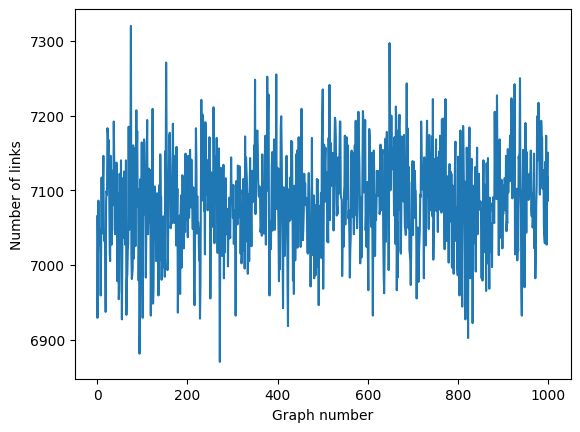
\includegraphics[scale=0.4]{img/metropolis/corrected model/num_links_corrected.png}
    \caption{Number of links for every graph in the ensemble coming from the corrected model}
\end{figure}

\begin{figure}[!ht]
    \centering
    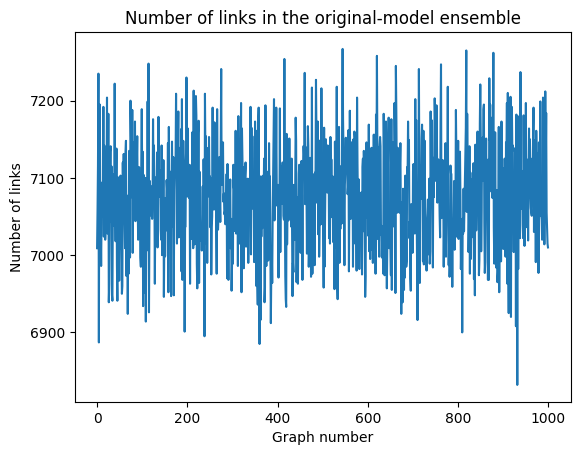
\includegraphics[scale=0.4]{img/metropolis/num_links_vanilla.png}
    \caption{Number of links for every graph in the ensemble coming from the corrected model}
\end{figure}

\clearpage
\textbf{Degrees, ANND}
\begin{figure}[!ht]
    \centering
    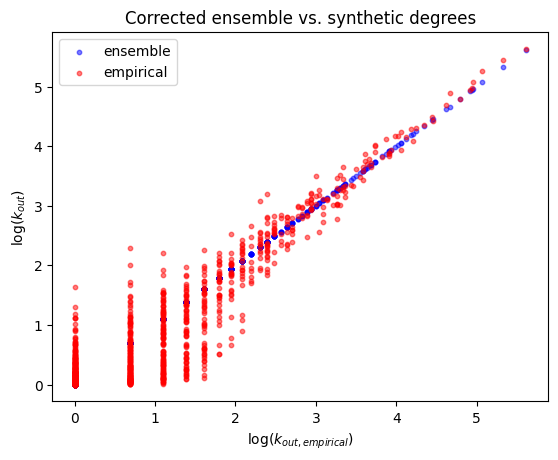
\includegraphics[scale=0.4]{img/metropolis/corrected model/dg_vs_dg.png}
    \caption{Degrees of nodes compared for the synthetic network and ensemble from the \textbf{corrected} model}
\end{figure}\begin{figure}[!ht]
    \centering
    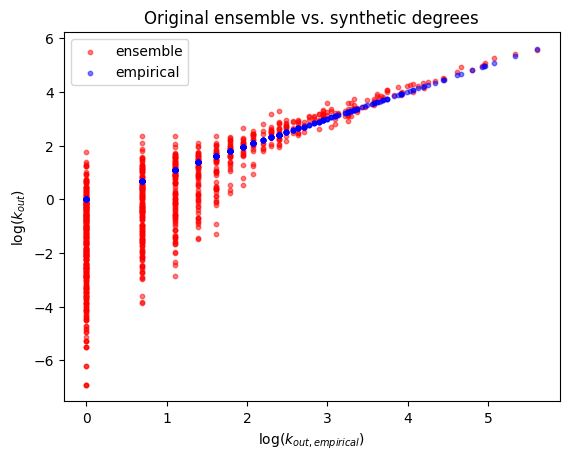
\includegraphics[scale=0.4]{img/metropolis/vanilla model/dg_vs_dg.png}
    \caption{Degrees of nodes compared for the the synthetic network and ensemble from the \textbf{original} model}
\end{figure}

\begin{figure}[!ht]
    \centering
    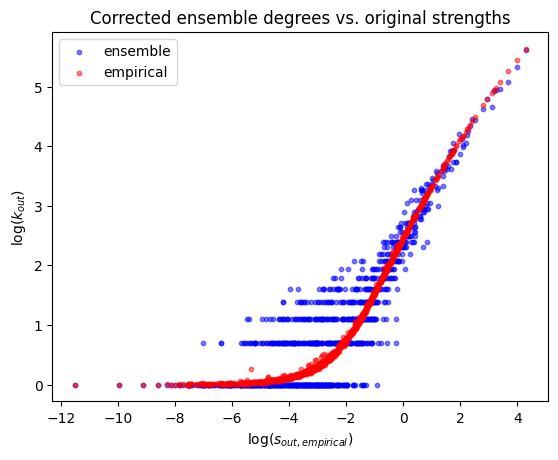
\includegraphics[scale=0.4]{img/metropolis/corrected model/dg_vs_s.png}
    \caption{Degrees of nodes compared for the the synthetic network and ensemble from the \textbf{corrected} model, now with strengths of the synthetic network on the x-axis.}
\end{figure}\begin{figure}[!ht]
    \centering
    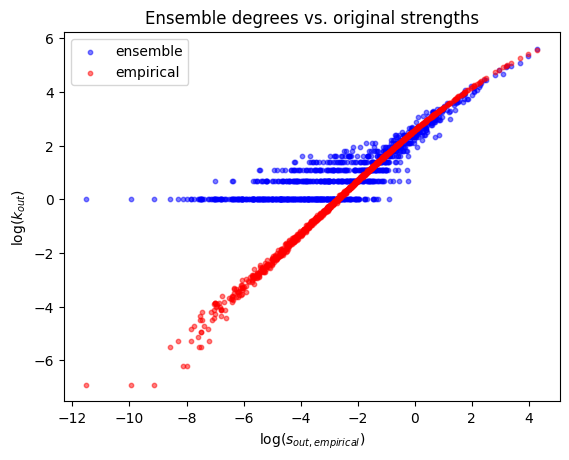
\includegraphics[scale=0.4]{img/metropolis/vanilla model/dg_vs_s.png}
    \caption{Degrees of nodes compared for the the synthetic network and ensemble from the \textbf{original} model}
\end{figure}

\begin{figure}[!ht]
    \centering
    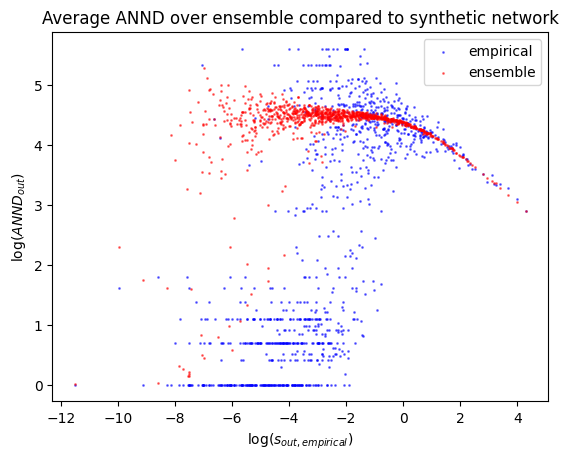
\includegraphics[scale=0.4]{img/metropolis/corrected model/annd_vs_s.png}
    \caption{Average nearest neighbor degree of the \textbf{corrected} model compared with the synthetic network, with strengths of the synthetic network on the x-axis.}
\end{figure}\begin{figure}[!ht]
    \centering
    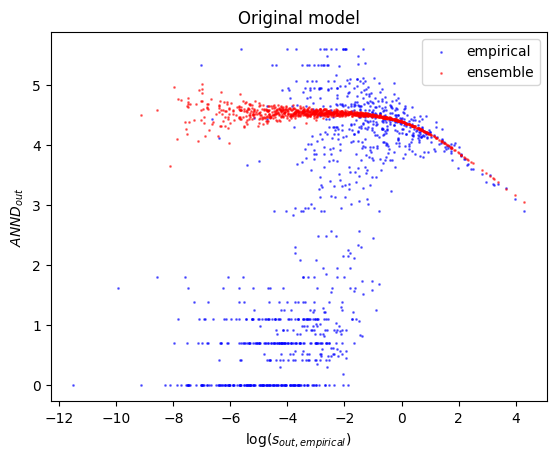
\includegraphics[scale=0.4]{img/metropolis/vanilla model/annd_vs_s.png}
    \caption{Average nearest neighbor degree of the \textbf{original} model compared with the synthetic network, with strengths of the synthetic network on the x-axis.}
\end{figure}

\begin{figure}[!ht]
    \centering
    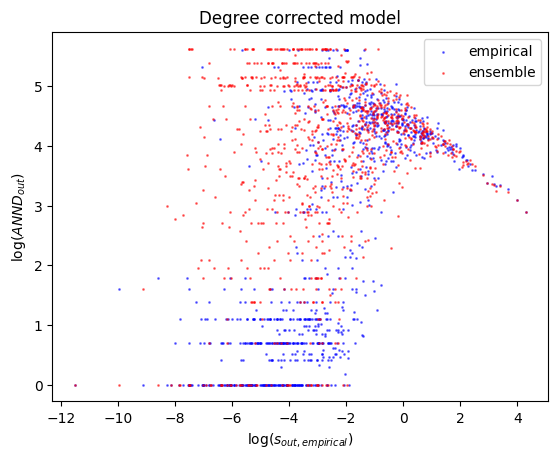
\includegraphics[scale=0.5]{img/metropolis/corrected model/annd_vs_s_sample.png}
    \caption{Average nearest neighbor degree of \textbf{one sample} of the \textbf{corrected} model compared with the synthetic network, with strengths of the synthetic network on the x-axis.}
\end{figure}\begin{figure}[!ht]
    \centering
    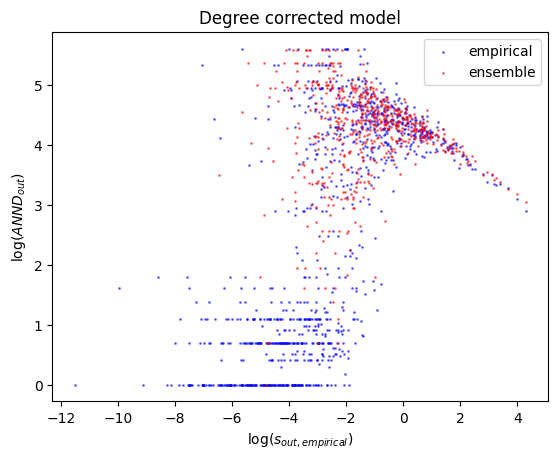
\includegraphics[scale=0.5]{img/metropolis/vanilla model/annd_vs_s_sample.png}
    \caption{Average nearest neighbor degree of \textbf{one sample} of the \textbf{original} model compared with the synthetic network, with strengths of the synthetic network on the x-axis.}
\end{figure}

\clearpage
\textbf{Strengths}

We can see that we systematically undervalue the strengths of nodes, which have low strength in the empirical graph. {\color{red} This could be a mistake in determining the strengths.}
\begin{figure}[!ht]
    \centering
    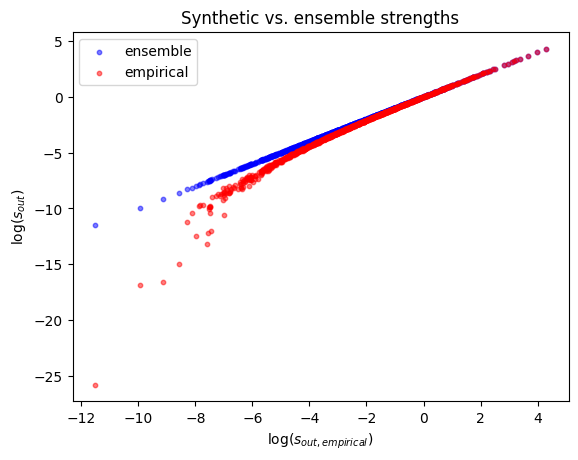
\includegraphics[scale=0.5]{img/metropolis/corrected model/s_vs_s.png}
    \caption{Out-trengths of the \textbf{corrected} model compared with the synthetic network, with strengths of the synthetic network on the x-axis.}
\end{figure}\begin{figure}[!ht]
    \centering
    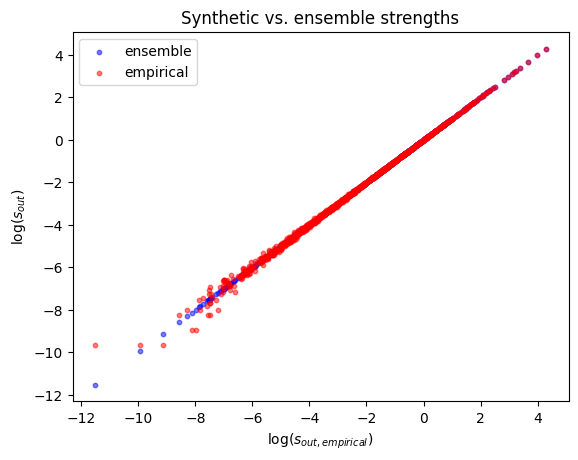
\includegraphics[scale=0.5]{img/metropolis/vanilla model/s_vs_s.png}
    \caption{Out-trengths of the \textbf{original} model compared with the synthetic network, with strengths of the synthetic network on the x-axis.}
\end{figure}


\end{document}
